%% A simple branched neurons.
\documentclass[crop,tikz]{standalone}
\usetikzlibrary{decorations}
\usetikzlibrary{decorations.pathmorphing}
\usetikzlibrary{intersections}
\begin{document}

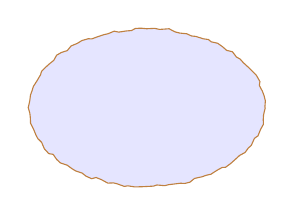
\begin{tikzpicture}[scale=1
    , every node/.style={}
    ]

    \node[] (soma) at (0,0) {}; 
    % Now draw a axon
    \path[blue!10
        , draw = brown
        , decorate
    ] (soma) -- +(1,0); 

    %% Here we go.
    \fill[blue!10
        , draw=brown
        , decorate
        , decoration={random steps, segment length=2, amplitude=0.5}
        , name path = somap
    ] (soma) ellipse (1.5 and 1);
%%    \node[draw
%%        , circle
%%        , decorate
%%        , decoration={random steps, segment length=1, amplitude=1}
%%    ] (soma) at (3, 0) {};
    
\end{tikzpicture}    

\end{document}

